\section{Busauslastung messen}
Um zu beurteilen, ob Bluetooth Low Energy (BLE) eine geeignete Lösung für die Übertragung von Telegrammen vom Sniffer zum Endgerät darstellt, wurde die Busauslastung mittels Oszilloskop aufgezeichnet und mittels Matlab ausgewertet. Ziel war es, abzuschätzen, ob die dabei gewonnenen effektiven Nutzdaten über BLE übertragen werden können. Gleichzeitig gilt es darum, die ersten Erfahrungen im Bereich der Signalauswertung zu gewinnen und diese im Bereich des FPGA's gewinnbringend einzusetzen.

Für die Analyse wurden zwei Messungen durchgeführt: Eine unter Normallast und eine unter Volllast. Die Volllast wurde simuliert, indem der Depot-Diagnosespeicher (abk. DDS) auf dem Fahrzeugdisplay abgerufen wurde. Dies führte dazu, dass der Speicher die entsprechenden Daten über den Bus an das Display sendete, was kurzfristig zu einer höheren Auslastung führte.

Die Messungen wurden mit einem Picoscope 2207B durchgeführt, während die anschliessende Auswertung mit MATLAB realisiert wurde.

\subsection{Messaufbau}

Der Messaufbau ist in Abbildung \ref{fig:MessaufbauBusauslastungMessen} dargestellt. Um die Busauslastung zu messen, wurde die MVB-Leitung, die normalerweise von Gerät zu Gerät durchgeschleift ist, an einer geeigneten Stelle unterbrochen und ein Leitungsaufteiler eingefügt. Dies ermöglichte den direkten Zugriff auf die differentiellen Leitungen des Busses mit dem Picoscope. Der MVB-Loop wurde dabei wieder geschlossen, sodass keine Geräte vom Bus abgetrennt wurden. Die gemessenen Daten wurden über eine USB-Schnittstelle an einen Laptop übertragen und dort mit der Pico-Software aufgezeichnet.

\begin{figure}[H]
    \centering
    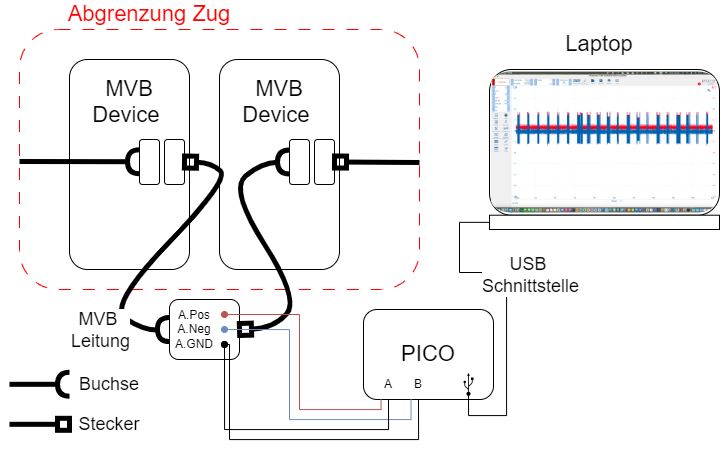
\includegraphics[width=0.8\linewidth]{Figures/Chap3/Busauslastung/Messaufbau_PICO_IC2000.png}
    \caption{Messaufbau Busauslastung messen}
    \label{fig:MessaufbauBusauslastungMessen}
\end{figure}

Die erfassten Daten wurden anschliessend in das MATLAB-Dateiformat (.mat) exportiert. Die Struktur der MATLAB-Datei ist in Abbildung \ref{fig:MatlabFileStruktur} dargestellt. Die Variablen \textit{A} und \textit{B} entsprechen den Messpunkten des Picoscope, während \textit{Tinterval} die Zeit zwischen zwei Messpunkten angibt. 

\begin{figure}[H]
    \centering
    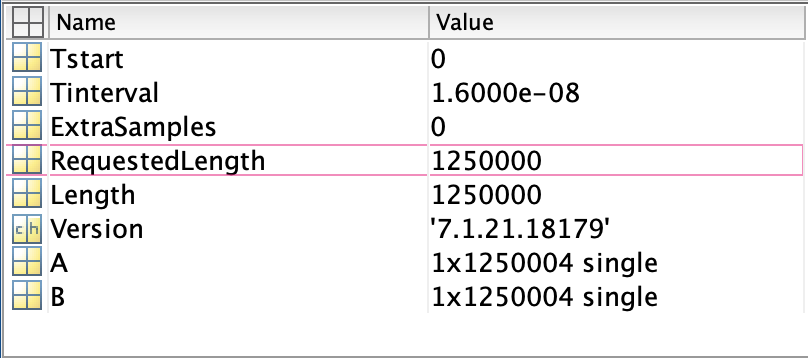
\includegraphics[width=0.5\linewidth]{Figures/Chap3/Busauslastung/Matlab_file_struktur.png}
    \caption{Matlab File Struktur}
    \label{fig:MatlabFileStruktur}
\end{figure}

Der Messaufbau blieb für die Messungen unter Normallast und Volllast identisch. Um die Volllast zu simulieren, wurde der Befehl zur Anzeige der Depot-Diagnosedaten auf dem Fahrzeugdisplay ausgelöst, bevor die Messung gestartet wurde. Der Zeitraum zwischen der Eingabe des Befehls und der Darstellung der Daten auf dem Display beträgt etwa 5 Sekunden.

\subsection{Einstellung Osziloskop}
Das Picoscope-Osziloskop wurde entsprechend der Anforderungen für die Messung wie folgt eingestellt: Die Abtastrate wurde auf 62.5 MS/s eingestellt, wodurch sich ein Abtastintervall von 16ns ergibt. Somit ist sichergestellt, dass jedes Machester-Bit mit jeweils 40 Punkten abgetastet wird (siehe Kapitel \ref{sub:BitEncoding}). Mit dem verfügbaren Speicher des Picoscope lassen sich somit 25 Messungen mit einer Messdauer von 20ms speichern.

\subsection{Matlab Auswertung}
Die Auswertung der Analogwerte wurde mit Matlab realisiert. Ziel war es herauszufinden, wie gross die Busauslastung in Bits/s ist. Für die Übertragung mit Bluetooth waren nur die Master Frame Daten und die Master Check Sequenz (siehe Kapitel \ref{sub:MasterFrame}) sowie die Slave Frame Daten und die Slave Check Sequenzen (siehe Kapitel \ref{sub:SlaveFrame}) von Interesse. Der Overhead der Start- sowie der Enddelimiter müssen entfernt werden. 

\subsubsection{Variablen initialisieren}
%\textcolor{red}{Zeitvektor initialisiert, damit Signal im Zeitbereich geplotet werden konnte. Analyse des Signals möglich. Einbindung Plot!}
Die mit Picoscope generierten Matlab Dateien konnte das Signal im Zeitbereich grafisch dargestellt werden. Der unten dargestellte Code zeigt, wie die Abbildung \ref{fig:MvbOhneDds} erstellt wurde. Die Abbildung \ref{fig:MvbMitDds} wurde mit dem anderen Datenset und einem angepassten Titel erstellt. 

\begin{lstlisting}[language=Matlab]
load("Messung ohne DDS/20240930-0002_01.mat")
%load("Messung mit DDS/20240930-0004_18.mat")

% ---- Variabeln initialisieren --------
N_org = length(A);          
Ts = Tinterval;             % gegeben von .mat
t_org = [0:N_org-1]*Ts;     % erstellung Zeitvektor

figure()                    % neuer Plot erstellen
plot(t_org, C)
title("MVB Signal ohne DDS im Zeitbereich (1 von 25)")
legend("MVB")
axis([0 0.02 -7 7])

% ----- PLOTS ----------------
plot(t_org, C)              % Plot Signal im Zeitbereich
\end{lstlisting}

\begin{figure}[H]
    \centering
    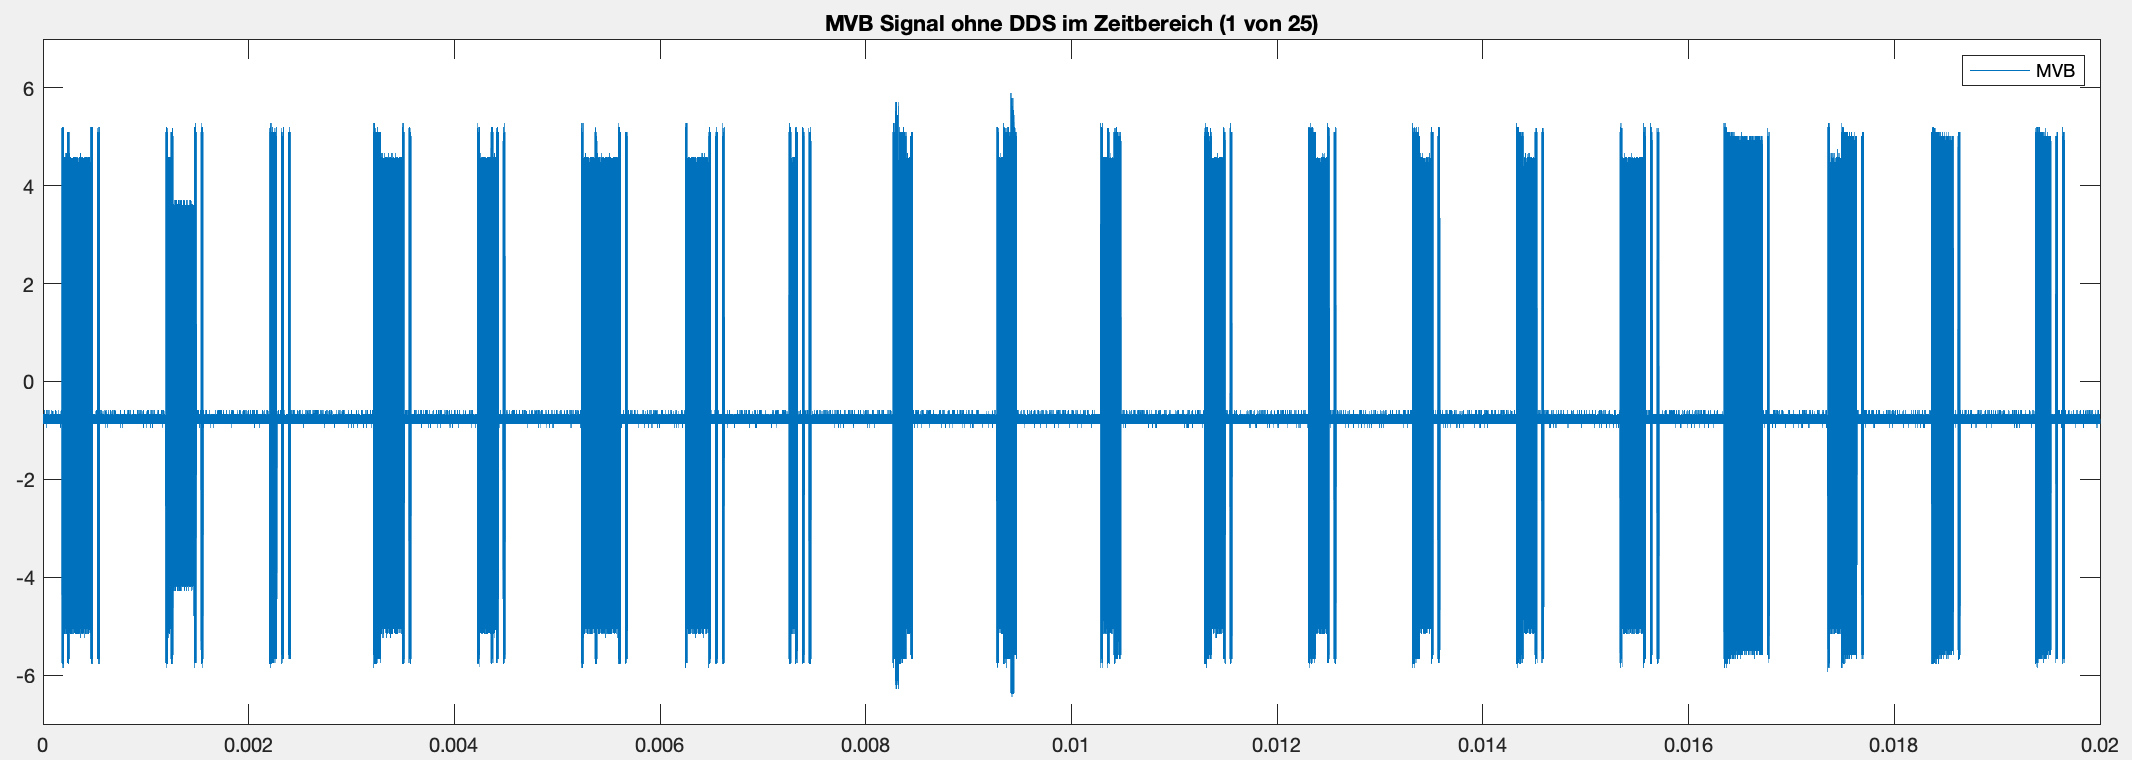
\includegraphics[width=0.8\linewidth]{Figures/Chap3/Busauslastung/MVB_Signal_ohneDDS.png}
    \caption{MVB Signal ohne DDS, Aufzeichnung 1 von 25}
    \label{fig:MvbOhneDds}
\end{figure}

\begin{figure}[H]
    \centering
    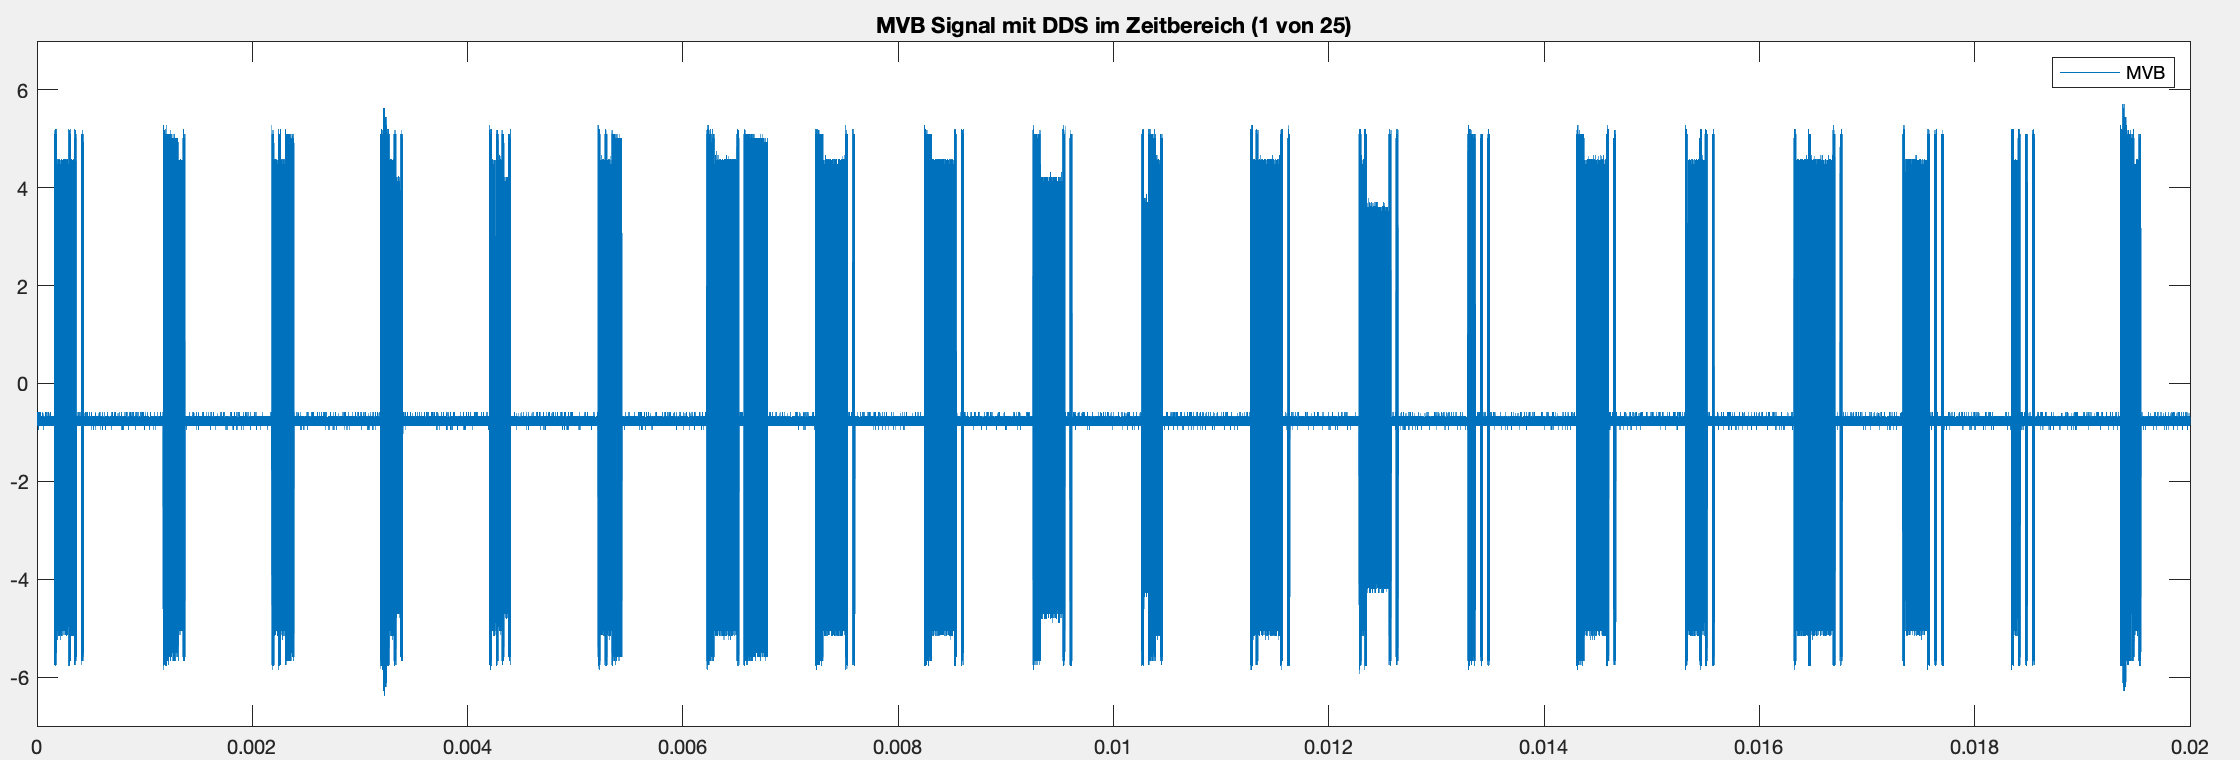
\includegraphics[width=0.8\linewidth]{Figures/Chap3/Busauslastung/MVB_Signal_mitDDS.png}
    \caption{MVB Signal mit DDS, Aufzeichnung 1 von 25}
    \label{fig:MvbMitDds}
\end{figure}

Zu sehen sind Zeitbereiche, in denen Daten ausgetauscht werden gefolgt von einem Zeitbereich, in dem sich der Bus in einem Idle Zustand befindet. Ebenfalls bemerklich ist, dass von blosem Auge der Unterschied zwischen Volllast (mit DDS) und Normallast (ohne DDS) nicht zu erkennen ist.

\subsubsection{Delimiter erkennen}
%\textcolor{red}{Anzahl delimiter erkennen. Charakteristik erkannt -> letzte werte Idle, dann Nulldurchgang, aber nur wenn einer der nächsten 20 Werte über null ist, sonst wurde peak am schluss auch gezählt. }
Um die Start-Delimiter zu erkennen, wurde die Charakteristik eines Delimiters gemäss Kapitel \ref{sub:StartDelimiter} untersucht. In Abbildung \ref{fig:AusschnittMvbOhneDds} wurde der Zeitbereich vergrössert. Dadurch lassen sich die Telegramme (gemäss Kapitel \ref{sub:MasterSlavePrinzip}) besser sehen.

\begin{figure}[H]
    \centering
    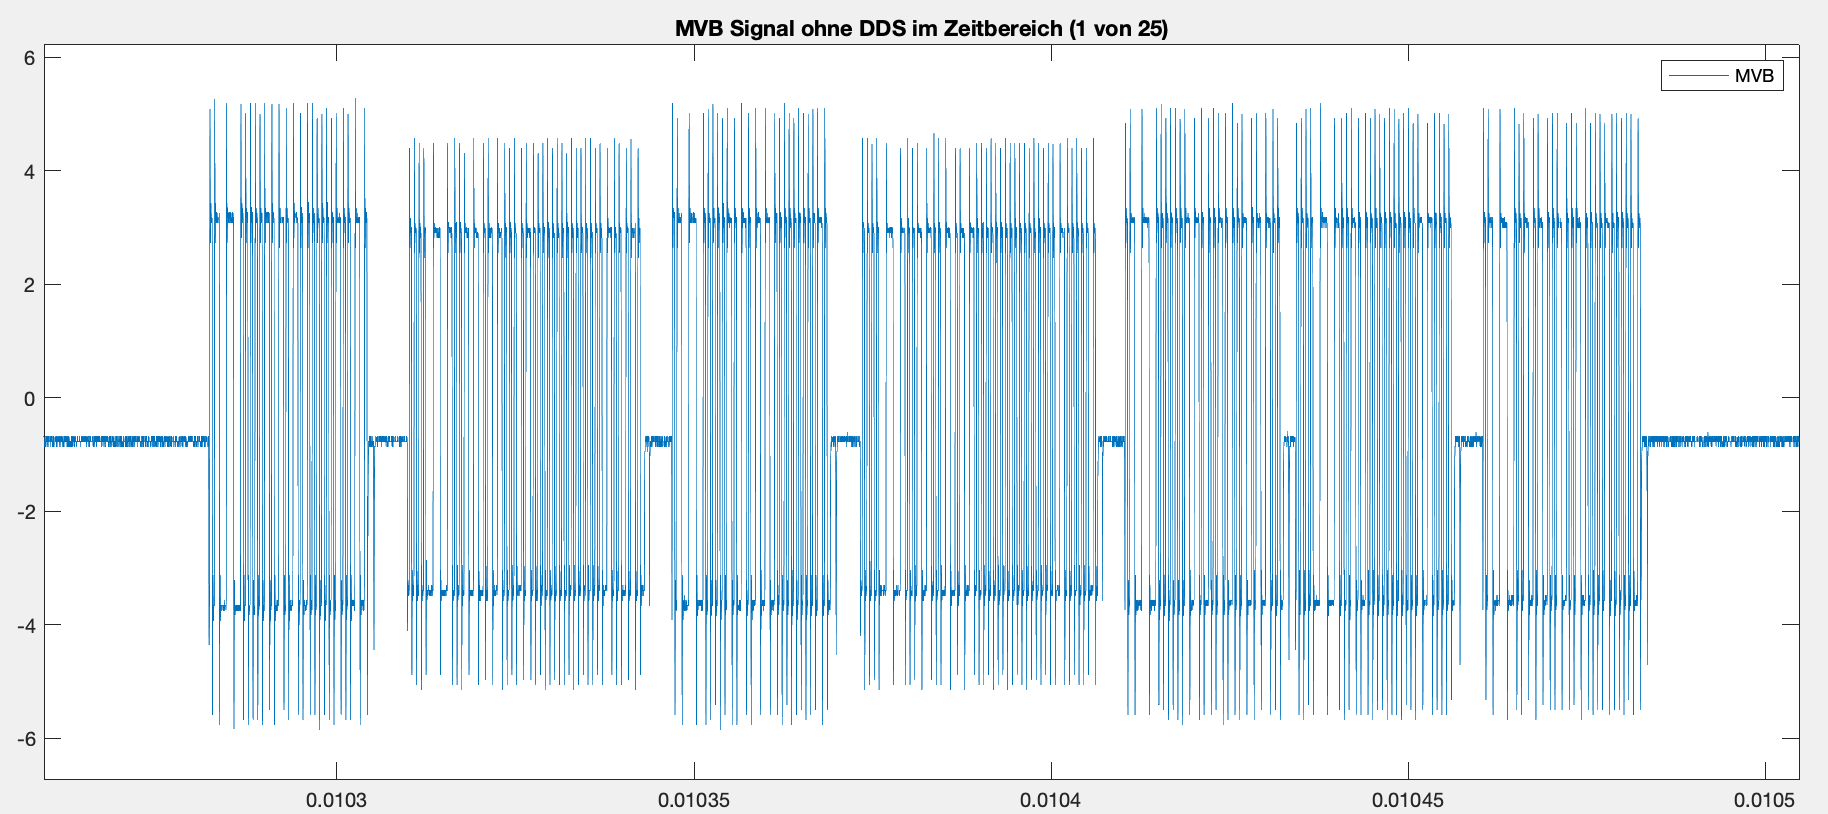
\includegraphics[width=0.9\linewidth]{Figures/Chap3/Busauslastung/Ausschnitt_MVB_ohneDDS.png}
    \caption{Ausschnitt MVB Signal ohne DDS}
    \label{fig:AusschnittMvbOhneDds}
\end{figure}

Zu sehen ist, dass vor jedem Startbit (Master- und Slave-Frame) das Signal eine gewisse Zeit Idle signalisiert, bevor das Startbit eine negative Flanke auslöst. Das kann verwendet werden, um das Startbit zu erkennen. In einem Array mit 20 Werten sollen alle Werte im Idle Bereich liegen (zwischen -0.5 und -1 V) und die nächste negative Flanke, also ein Wert unter -1 wird als Start detektiert. Für die Ausgabe auf dem Plot wurden die Spannungs- und Zeitpunkte gespeichert und dem Plot hizugefügt. Abbildung \ref{fig:MVBDelimiterFalsch} zeigt diesen Plot.

\begin{lstlisting}[language=Matlab]
detected_values = [];
detected_times = [];
delimiter = 0;

n_samples = 20;

for i = n_samples+1:length(C)
    % Ueberpruefen, ob die letzten 20 Werte zwischen -0.5 und -1 liegen
    if all(C(i-n_samples:i-1) > -1 & C(i-n_samples:i-1) < -0.5)

        % Wenn der naechste Wert kleiner als -1.0 ist
        if C(i) < -1.0
            % Zaehler erhoehen
            delimiter = delimiter + 1;
                
            % Speichern des Werts und des entsprechenden Zeitwerts
            detected_values = [detected_values, C(i)];
            detected_times = [detected_times, t_org(i)];
        end
    end
end
\end{lstlisting}

\begin{figure}[H]
    \centering
    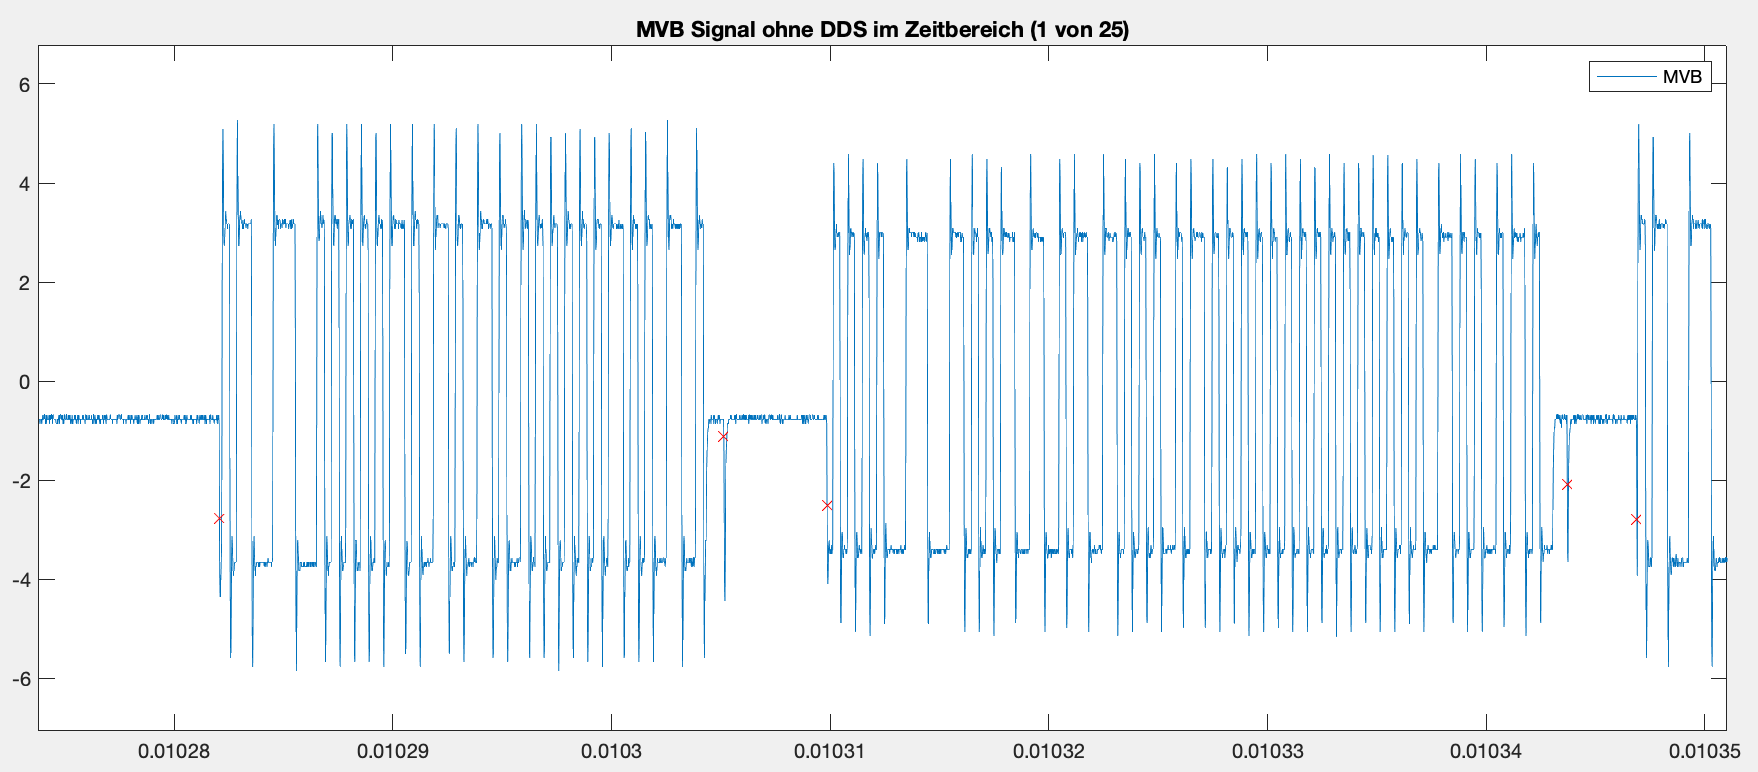
\includegraphics[width=0.9\linewidth]{Figures/Chap3/Busauslastung/Ausschnitt_MVB_Delimiter_falsch.png}
    \caption{Ausschnitt der MVB Messung ohne DDS mit nicht korrekter Delimiter erkennung}
    \label{fig:MVBDelimiterFalsch}
\end{figure}

Wird der Zeitbereich erneut vergrössert, ist zu sehen, dass am Ende eines Master- oder Slave-Frame die Signalleitung in den negativen Bereich gezogen wird, was zu einer falschen erneuten Detektion eines Start-Delimiters führt.

Das Startbit hat gemäss Kapitel \ref{sub:StartDelimiter} die Eigenschaft, dass es während der ersten Hälfe der Bitdauer High und in der zweiten Hälfte Low ist. Dies kann als Bedingung für die Erkennung der eines Start-Delimiters einfliessen. Dies wurde im Code so implementiert, dass nach der Erkennung der negativen Flanke zusätzlich abgefragt wurde, ob einer der nächsten 20 Werte (also 333ns) ein Wert über 0V gemessen wurde. Der wurde Code wie folgt angepasst und der daraus entstandene Plot ist in Abbildung \ref{fig:DelimiterRichtig} zu sehen.

\begin{lstlisting}[language=Matlab]
detected_values = [];
detected_times = [];
delimiter = 0;

n_samples = 20;

for i = n_samples+1:length(C)
    % Ueberpruefen, ob die letzten 20 Werte zwischen -0.5 und -1 liegen
    if all(C(i-n_samples:i-1) > -1 & C(i-n_samples:i-1) < -0.5)

        % Wenn der naechste Wert kleiner als -1.0 ist
        if C(i) < -1.0

            % Wenn einer der naechsten 20 Werte ueber Null ist, ist es ein Start Delimiter
            if any(C(i+1:i+20) > 0)
            
                % Zaehler erhoehen
                delimiter = delimiter + 1;
                    
                % Speichern des Werts und des entsprechenden Zeitwerts
                detected_values = [detected_values, C(i)];
                detected_times = [detected_times, t_org(i)];
                
            end
        end
    end
end
\end{lstlisting}

\begin{figure}[H]
    \centering
    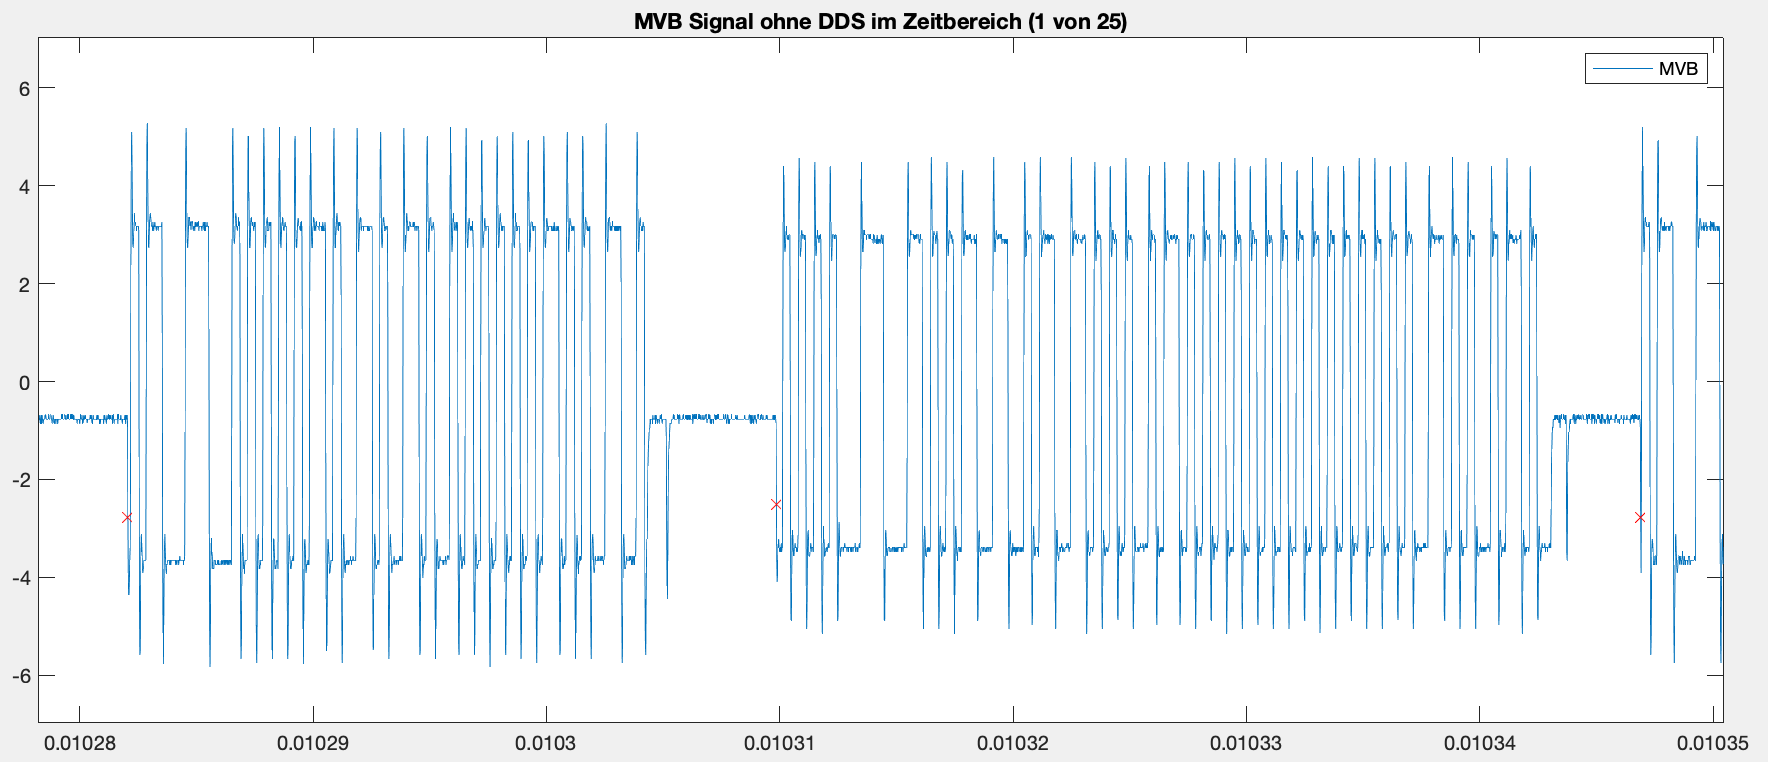
\includegraphics[width=0.9\linewidth]{Figures/Chap3/Busauslastung/Ausschnitt_MVB_Delimiter_richtig.png}
    \caption{Ausschnitt der MVB Messung ohne DDS, mit korrekter Start-Delimiter erkennung}
    \label{fig:DelimiterRichtig}
\end{figure}


\subsubsection{Nulldurchgänge}
\label{subsub:Nulldurchgänge}
%\textcolor{red}{Anzahl bits mit Startdelimiter erkennen. Als erstes alle werte zwischen 0 und -1V gelöscht, weil Idle. Dann wurde eine Flanke detektiert. Wenn eine Flanke detektier um 30 Werte vorwärts springen (damit zweite Flange nicht nochmals erkennt wird (manchester encodiertes Signal)}
In diesem Schritt wurde mit Matlab versucht, die Anzahl Bits zu aus der Messung auszuwerten. Gemäss Kapitel \ref{sub:BitEncoding} gibt es für den Wert "'0"' und "'1"' jeweils einen Flankenwechsel in der Hälfte der Bitdauern (abk. BT und entspricht gemäss Kapitel \ref{sub:GeschwindigkeitDatenbus}: 1 BT = 666ns). Dies kann verwendet werden, um die Anzahl Bits herauszufinden. Anhand Abbildung \ref{fig:Suchalgo_Bits} kann der gewählte Suchalgorithmus erklärt werden.

\begin{figure}[H]
    \centering
    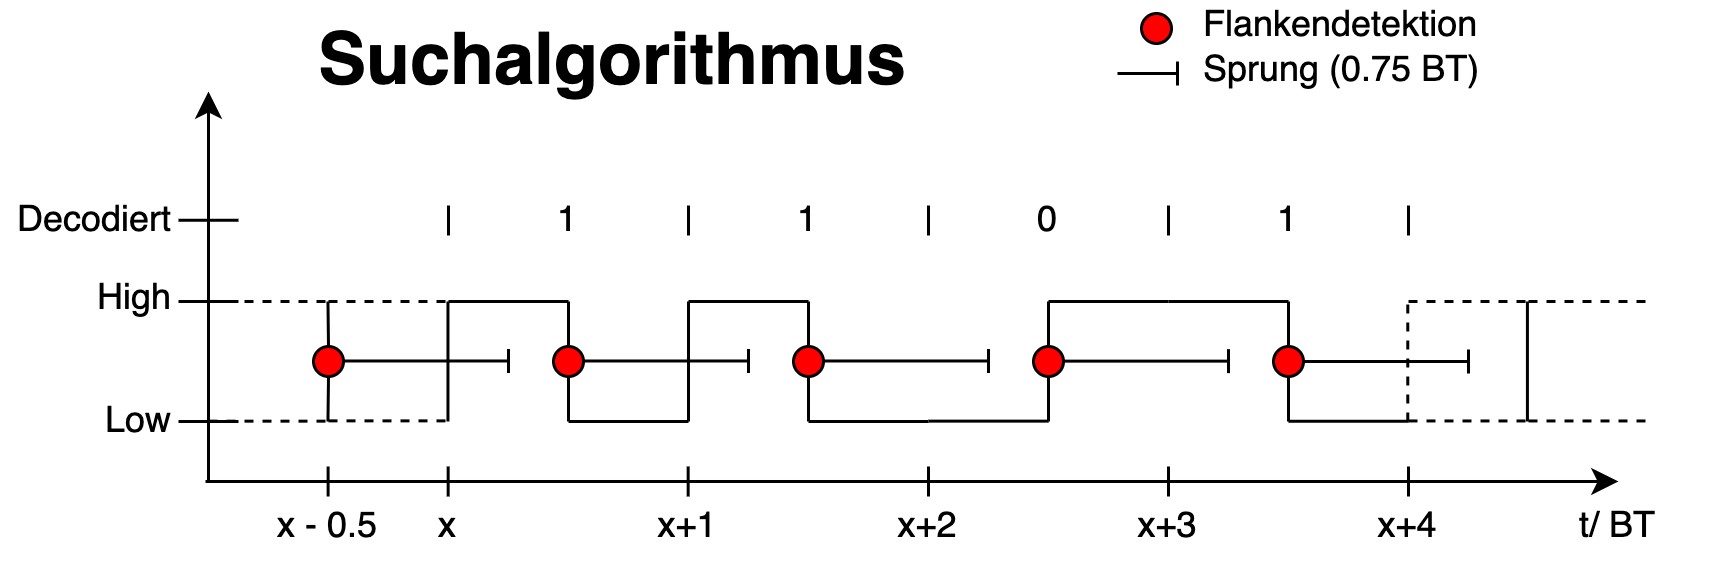
\includegraphics[width=0.9\linewidth]{Figures/Chap3/Busauslastung/Suchalgorithmus_Bits.png}
    \caption{Suchalgorithmus der Bits in einem Manchester encodierten Signal}
    \label{fig:Suchalgo_Bits}
\end{figure}

X steht dabei für einen zufälligen Zeitpunkt. Auf der Abszisse ist die Zeit in Bitdauer aufgetragen. Auf der Ordinate ist einmal ein Beispielsignal und die Decodierung vom Signal aufgezeigt. Da in der Mitte der Bitdauer eine Flanke zu erwarten ist, wird auch eine halbe Bitdauer vor X eine Flanke erwartet. Dies ist der Einstieg. Wird eine Flanke detektiert, wird um eine Bitdauer von 0.75 positiv in der Zeit gesprungen. Der Sprungpfeil zeigt mit seinem flachen Ende, ab wo die nächste Flanke gesucht wird. Der Sprung hat den Grund, dass Flankendetektionen, wie dieser bei \textit{x+1} in Abbildung \ref{fig:Suchalgo_Bits}, nicht gezählt werden, da diese die Auswertung verfälschen.

Gemäss Abbildungen \ref{fig:MasterStartdel} und \ref{fig:SlaveStartdel} sind die Anzahl Flanken, welche in einem Master Startdelimiter und einem Slave Startdelimiter gezählt werden gleich Sieben.

\begin{figure}[H]
    \centering
    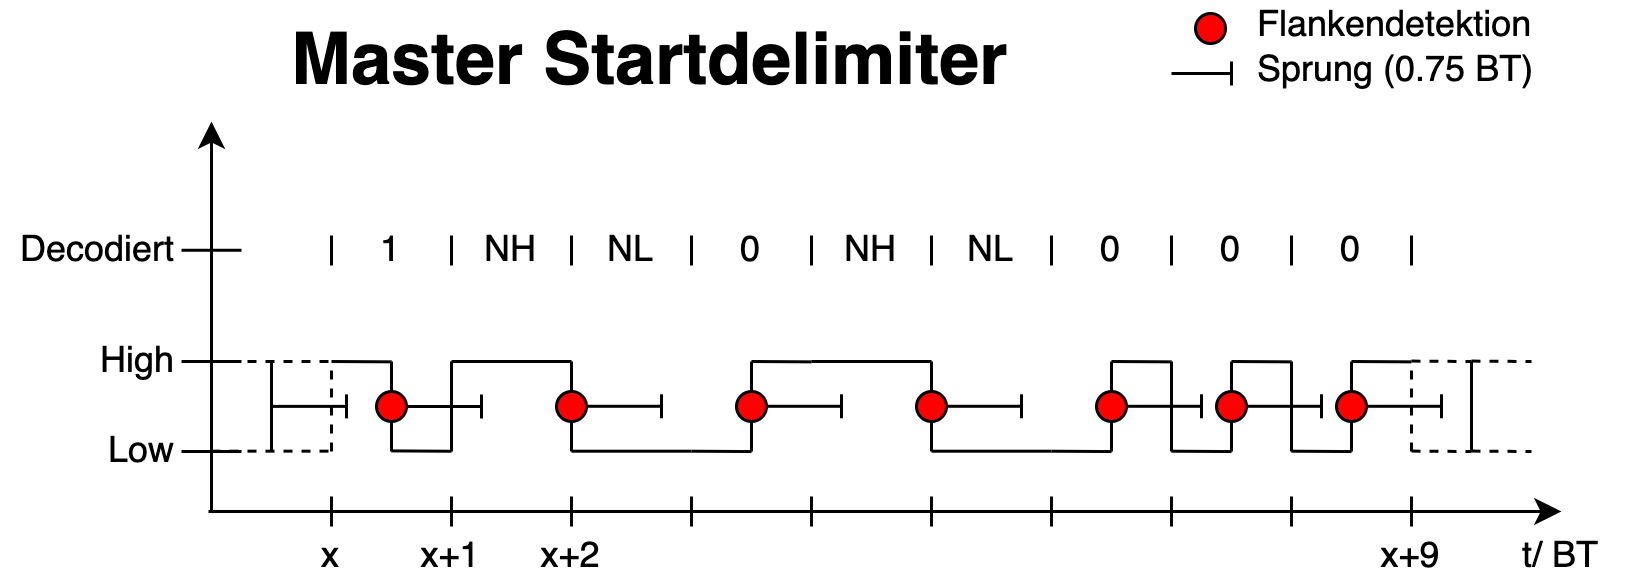
\includegraphics[width=0.9\linewidth]{Figures/Chap3/Busauslastung/Master_Startdel.png}
    \caption{Anzahl Flanken in einem Master Startdelimiter}
    \label{fig:MasterStartdel}
\end{figure}

\begin{figure}[H]
    \centering
    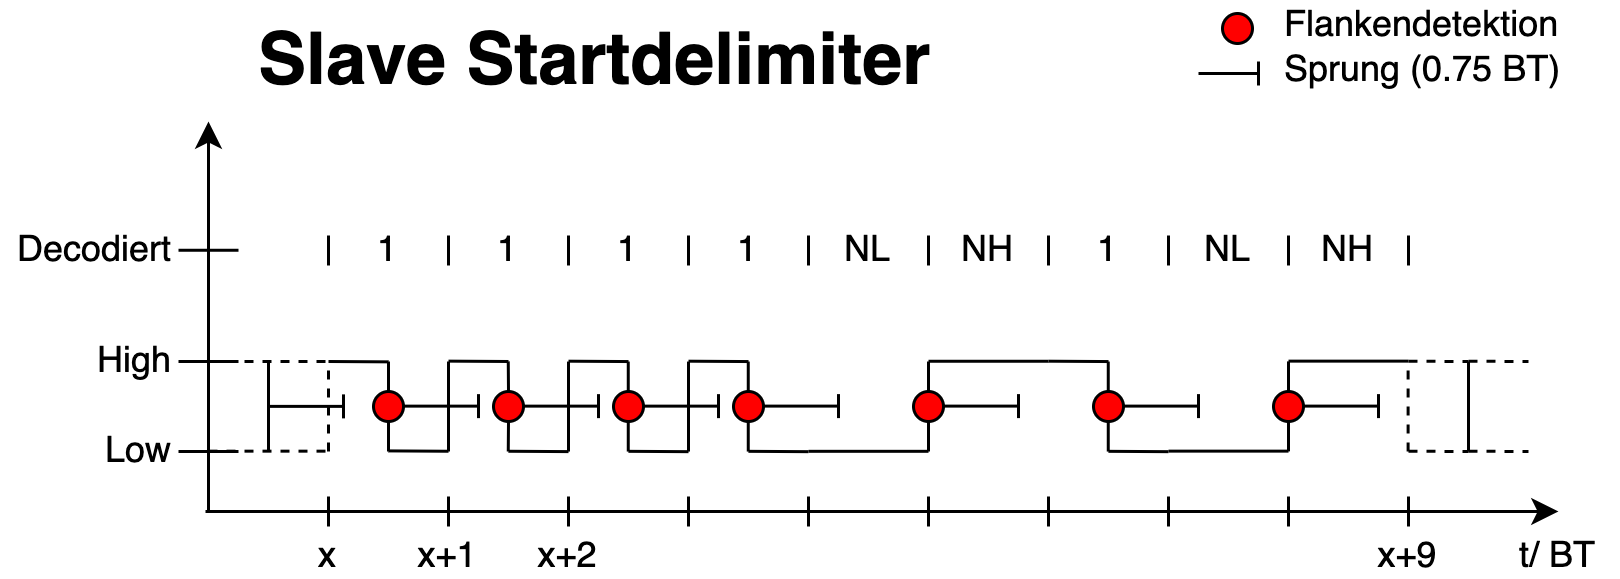
\includegraphics[width=0.9\linewidth]{Figures/Chap3/Busauslastung/Slave_Startdel.png}
    \caption{Anzahl Flanken in einem Slave Startdelimiter}
    \label{fig:SlaveStartdel}
\end{figure}


Für die Auswertung am MVB Signal wurde in einem ersten Schritt das Idle Signal, also alle Messpunkte zwischen -0.5 V und -1V aus dem Signal entfernt. Was daraus folgt, ist ein Signal, welches Startbits, Startdelimiter, Masterframe- sowie Slaveframe-Daten enthält. In Abbildung \ref{fig:ReineDaten} ein Vergleich zwischen beiden Signalen zu sehen. Oben mit Idle Signal, unten ohne Idle Signal.

\begin{figure}[H]
    \centering
    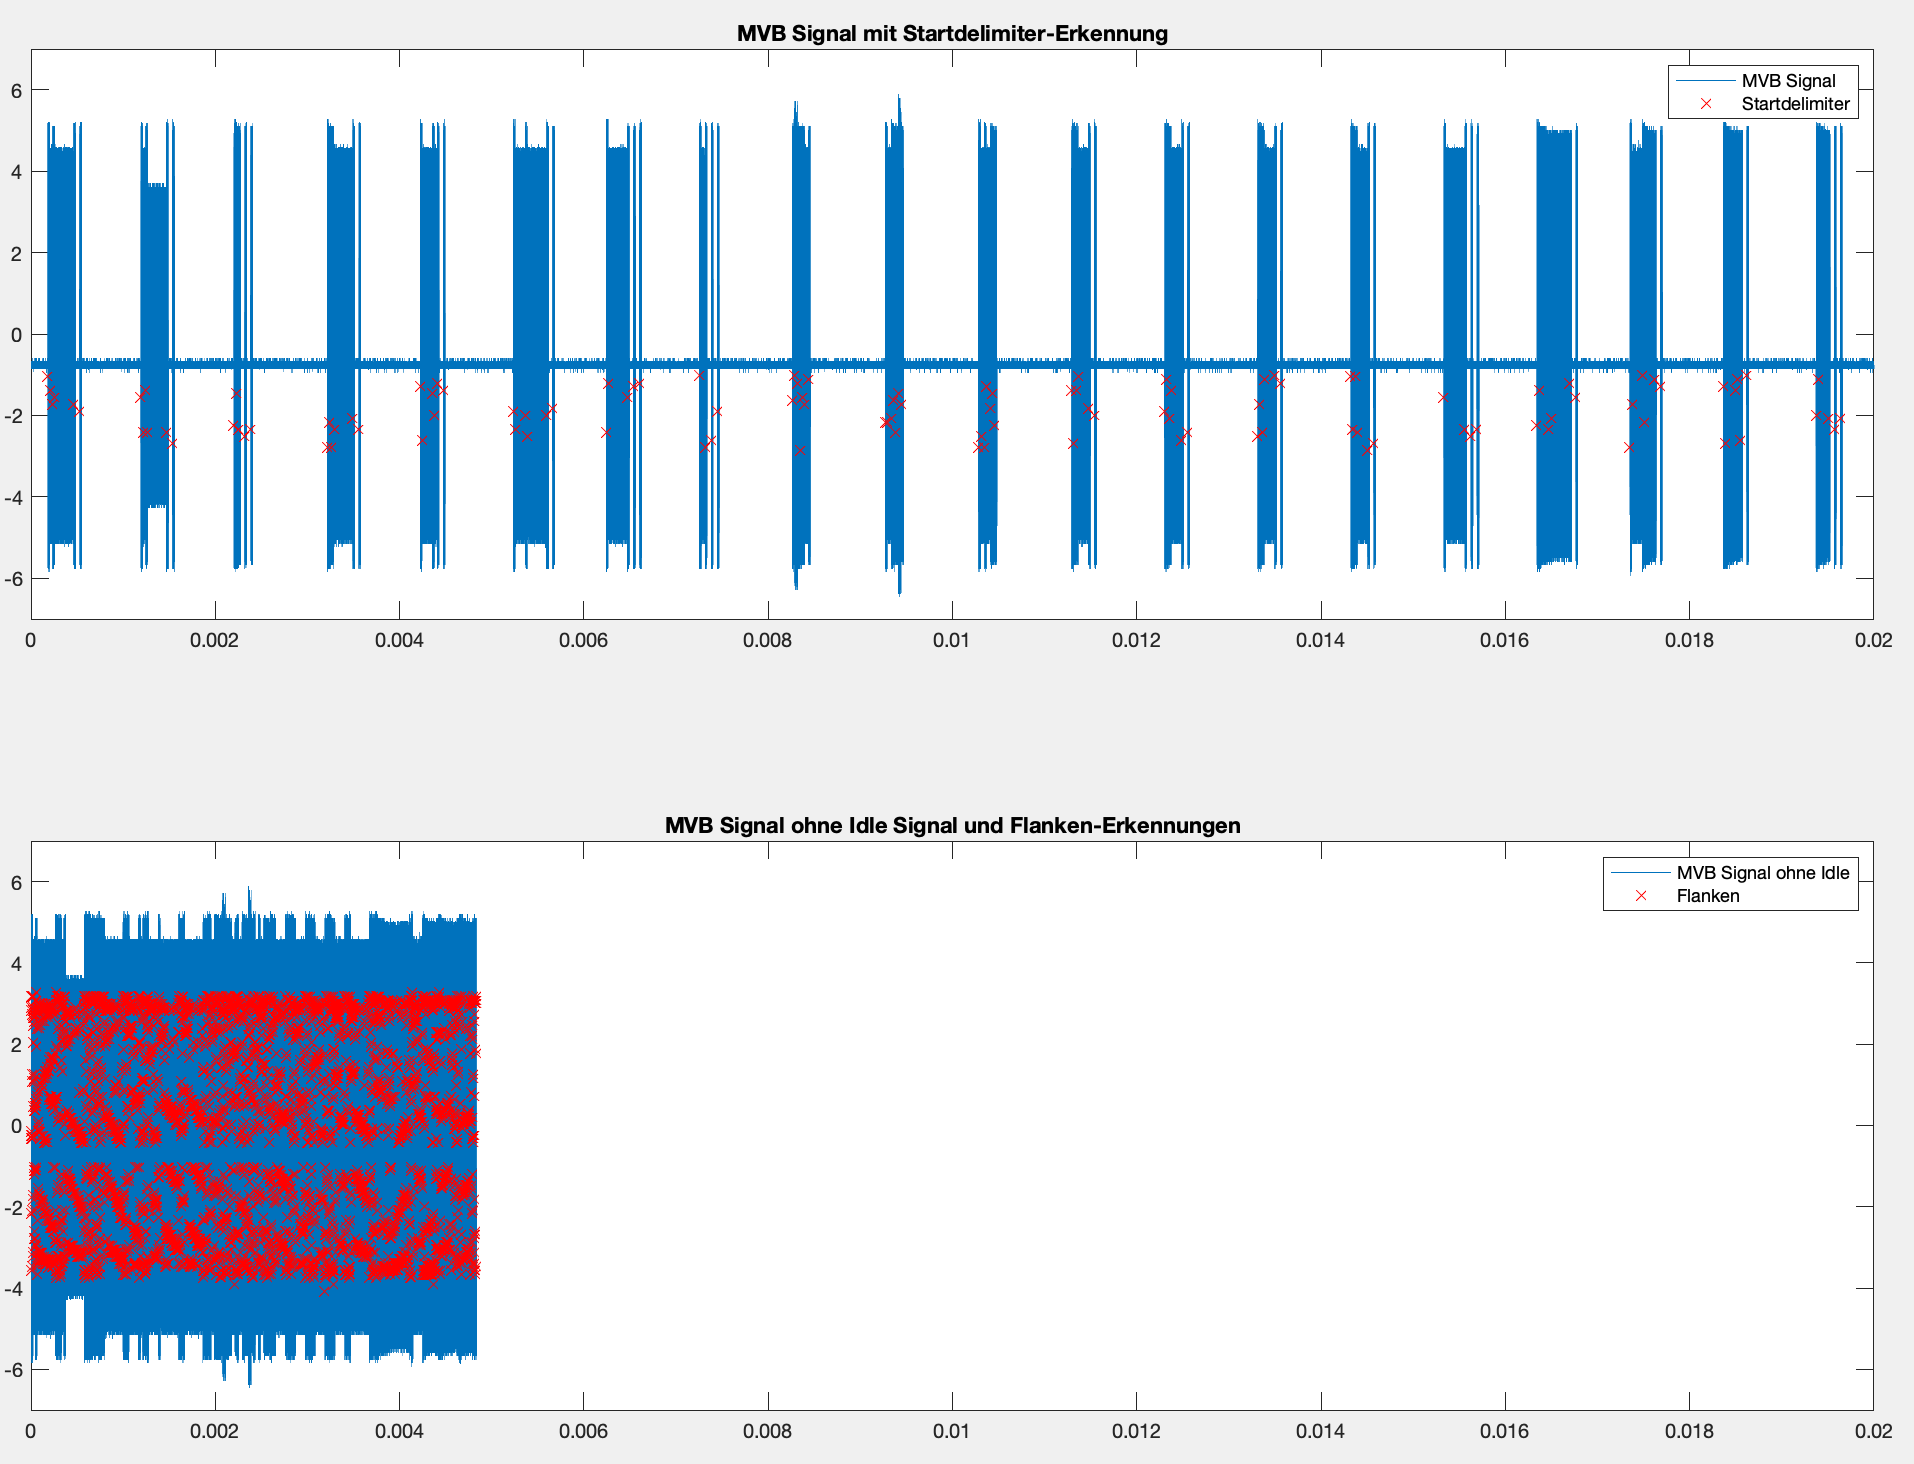
\includegraphics[width=0.75\linewidth]{Figures/Chap3/Busauslastung/Vergleich_MVB_mit_ohne_Idle.png}
    \caption{Vergleich MVB Signal mit und ohne Idle Signal über einen Zeitraum von 20ms}
    \label{fig:ReineDaten}
\end{figure}

Der Suchalgorithmus wurde in Matlab gemäss dem nachfolgenden Code implementiert

\begin{lstlisting}[language=Matlab]
% ---- Nulldurchgaenge ---------------

% Aus dem Sigal, nehme alle Werte ausser das Idle Signal (~ -0.75V)
data_ohne_idle = C(C > -0.5 | C < -1);

% neuer Zeitvektor initalisieren
N_fil = length(data_ohne_idle);
t_fil = [0:N_fil-1]*Ts;

% Zaehlervariablen initialisieren
z_num = 0; % Zaehlervariable fuer bit == flanken
used_i = [];

% Starte bei Index 10, damit wird erste Fanke des Startbits uebersprungen
i = 10; 


while i < N_fil

    % Positive Flanke erkennen
    if data_ohne_idle(i) < 0.75 && data_ohne_idle(i+1) > 0.75

        % Fuer Ausgabe in Plot speichern
        used_i = [used_i , i];
        z_num = z_num + 1; 

        % Ueberspringe Manchester Flankenwechsel ( 333ns < t < 666ns; ts = 16ns --> i = i + 20...40)
        i = i + 30; 

    % Negative Flanke erkennen
    elseif data_ohne_idle(i) > 0.75 && data_ohne_idle(i+1) < 0.75

        % Fuer Ausgabe in Plot speichern
        used_i = [used_i , i]; 
        z_num = z_num + 1;

        % Ueberspringe Manchester Flankenwechsel ( 333ns < t < 666ns; ts = 16ns --> i = i + 20...40)
        i = i + 30; 
       
    % Wenn keine Flanke erkennt wird um 1 erhoehen
    else
        i = i + 1;
    end
end
\end{lstlisting}




\subsubsection{Auswertung Effektive Nutzdaten}
%\textcolor{red}{Effektive = Anzahl Nuldurchgänge - (Delimiert * 9); Tablle effiktive Nutzwerte mit und ohne DDS.}
Nun wurde ausgewertet, wie viele Bits in einer Zeitdauer von 20ms geschickt wurde und wie viele Startdelimiter in derselben Zeit erkennt wurden. Gemäss Kapitel \ref{subsub:Nulldurchgänge} ist sind die Master-Startdelimiter und Slave-Startdelimiter sieben Bits gross. Dies kann mit der Anzahl delimiter multiliziert werden und von der gesammtsumme der gezählen Bits abgezogen werden. Im nachfolgenden Code wird gezeigt, wie das in Matlab realisiert wurde.

\begin{lstlisting}[language=Matlab]
% --- Auswertung

dlm = delimiter * 7; % Delimiter bits (master/slave)
eff_bps = (z_num - dlm)/0.02; % Bits pro Sekunde effektive Nutzdaten

\end{lstlisting}

Die Busauslastung wurde für jede der je 25 Messungen für Normallast und Volllast durchgeführt. Der Matlabcode dazu ist im Anhang \ref{} zu finden. In Tabelle \ref{tab:Busauslastung} ist die Auswertung  der Busauslastung tabellarisch dargestellt. Die Spalten \textit{min} und \textit{max} sind jeweils die minimal sowie maximalen Werte der je 25 Messungen. Die Spalte \textit{mean} wurde mit dem Matlabbefehl \textit{mean()} berechnet und gibt den Mittelwert über die je 25 Messungen aus. 

\begin{table}[H]
    \centering
    \begin{tabular}{r|c|c|c}
        & min in Bits/s & mean in Bits/s & max in Bits/s\\ 
        \hline
        Normallast & 2.4705e+05 & 2.8823e+05 & 3.1885e+05\\
        \hline
        Volllast & 2.5935e+05 & 3.0456e+05 & 4.204e+05 \\
    \end{tabular}
    \caption{Busauslastung in Normallast und Volllast (ohne und mit DDS) }
    \label{tab:Busauslastung}
\end{table}
